% !TeX program = xelatex
\documentclass{vilgym}

% For math
\usepackage{mathtools}
\usepackage{amsfonts}

% For graphs
\usepackage{graphicx}

% General info
\title{Kunsti genereerimine teksti põhjal}
\authors{Karl-Joan Alesma, III MF}
\instructor{õp Malle Eglit}
\date{2019}

% Define expected value operator
\DeclareMathOperator{\EX}{\mathbb{E}}

\addbibresource{viited.bib}

\begin{document}
    \maketitle
    \tableofcontents

    \unsection{Definitsioonid}
    \begin{description}
		\let\originalitem\item
		\renewcommand*{\item}[1][]{\originalitem[#1]\label{def:#1}}

        \item{GAN} ing.k. \textit{generative adversarial network}
    \end{description}

	\newcommand*{\seedefinition}[1]{(\hyperref[def:#1]{vt~definitsiooni})}
    \newcommand*{\ingk}[1]{(\textit{ing. k. #1})}

    \unsection{Sissejuhatus}
    Sügavõppe on distsipliin, mis on eksisteerinud juba alatest 1940 aastatest (küll aga teise nime all), kuid on alles hiljuti kasvanud populaarsuses. Kiiret arengut ja edasi minekut on peamiselt põhjustanud kaks asja: arvuti ressursside kasv ning järjest suurenev andmete hulk. Need kaks asja on võimaldanud treenida sügavamaid, keerulisemaid ning täpsemaid mudeleid. \parencite{deeplearningbook}   

    Üks uus mudel, mis on kiire kasvuga tekkinud, on GAN ehk generatiivne adverstiivne võrk. Antud võrku on võimalik treenida jäljendama erinevaid andme distributsioone. Kasutades treenimise käigus õpitud representatsioone, suudab too võrk genereerida uut materjali, mis on sarnane treenimisel kasutatud andmetega. \parencite{gan}

    Uurimistöö eesmärk on luua mudel kasutades GANe, mis on ise võimeline genereerima kunsti teksti põhjal. Andes muldeli sisendiks kirjelduse, milline peab olema loodava kunstiteose sisu ja mis stiilis, genereerib mudel teose, mida tegelikkuses ei eksisteerigi. Lisaks saab autor selle protsessi käigus kinnitada ja laiendada oma teadmisi sügavõppest.

    Töö alguses annab autor ülevaate varasematest töödest selles valdkonnas ning tutvustab arenguid sügavõppes, mis on vajalikud töö mõistmiseks. See järel tutvustatakse erinevaid mudeleid, millele järgneb eksperimentaalne osa, kus analüüsitakse ning hinnatakse erinevate mudelite sooritust. 
    
    \section{Varasemad tööd}

    Uue materjali genereerimine on keeruline probleem. Kogu sügavõppes ajaloo vältelt on diskrimineerivad mudelid saavutanud paremaid tulemusi kui generatiivsed mudelid. Hiljuti on aga see muutunud GANide tekkega.

    GANid on saavutanud märkimisväärseid tulemusi pildi ja video generatsioonis ning ka super resolutsioonis. kunst

    tekst pildiks

    %  \section{Mudel}
    \section{Tehnilised detailid}
    \subsection{GAN}
    Generatiivne adversatiivne võrk ehk GAN \ingk{generative adversarial network} on sügavõppe mudel, mis koosneb kahest neruonvõrgust --- üks on diskrimineerija \ingk{discriminator} ja teine on generaator \ingk{generator}.  Generaatori ülesandeks on luua sisu, mis on sarnane kasutusel olevate andmete distributsiooniga. Diskrimineerija ülesandeks on määrata, kas talle näidatud sisu on võetud päris andmete hulgast või on loodud generaatori poolt.
    
    Generaatoril ja diskrimineerijal vastastikused ülesanded --- diskrimineerija proovib minimeerida viga, mis tehakse sisu klassifitseerimise käigus (kas on võetud päris andmete hulgast või loodud generaatori poolt), ja generaator proovib maksimeerida viga, mida diskrimineerija teeb klassifikatsiooni käigus. Kokkuvõtvalt need kaks võrku mängivad omavahel minimaksmängu \ingk{minimax}, mida võib võrrelda vägikaika veoga. Lõpuks jõutakse Nash tasakaalu \ingk{Nash equilibrium}, kus osalejatel ei ole enam midagi saada oma strateegia muutmisega \parencite{gametheory}. Ideaalis on sel juhul diskriminaatori poolt väljastatud tõenäosus  sõltumata sisendist $ 1/2 $.

    Ilustavalt võib mõelda generaatorist kui võltsjate meeskonnast, kes proovivad luua võltsraha ja kasutada seda ilma jäljeta. Diskrimineerija aga käitub kui politsei, proovides tuvastada kas tegu on võltsinguga. Alguses on võltsjatel võltsingud kehvad ning politseil on raskusi tuvastusega, aga aja jooksul muutuvad osapooled paremaks omavahelise võistluse tõttu, kuni hetkeni mil võltsingud pole enam eristatavad päris valuutast.

    Treenimis protsetuuri saab võtta kokku järgimse funktsiooniga:

    \begin{equation}
        \operatorname*{min}_G \operatorname*{max}_D V(D,G) = \EX_{\boldsymbol{x}\sim p_{andmed}(\boldsymbol{x})}[\log D(\boldsymbol{x})] + \EX_{\boldsymbol{z}\sim p_{\boldsymbol{z}}(\boldsymbol{z})}[\log(1-D(G(\boldsymbol{z})))]
    \end{equation}

    kus $ \boldsymbol{z} $ on müravektor, mis on võetud distributsioonist $ p_{\boldsymbol{z}} $ (nt. ühtlane- või normaaljaotus), $ \boldsymbol{x} $ on päris pilt, mis on võetud distributsioonist $ p_{andmed} $, $ G $ on generaator funktsioon ja $ D $ on diskrimineerija funktsioon. Praktikas võib juhtuda, et võrrandis nr 1 ei teki piisavalt tugevaid gradiente, et treenida $ G $-d. Selle asemel, et minimeerida $ \log (1 - D(G(\boldsymbol{z}))) $, saame panna $ G $ maskimeerima $ \log D(G(\boldsymbol{z})) $, mis tekkitab tugevamaid gradiente. Treenides $ G $ ja $ D $ vaheldumisi, treenitakse GANi looma pilte, mis sarnanevad andmete distributsiooniga. \parencite{gan}

    \subsection{CycleGAN}
    \begin{figure}
        \centering
            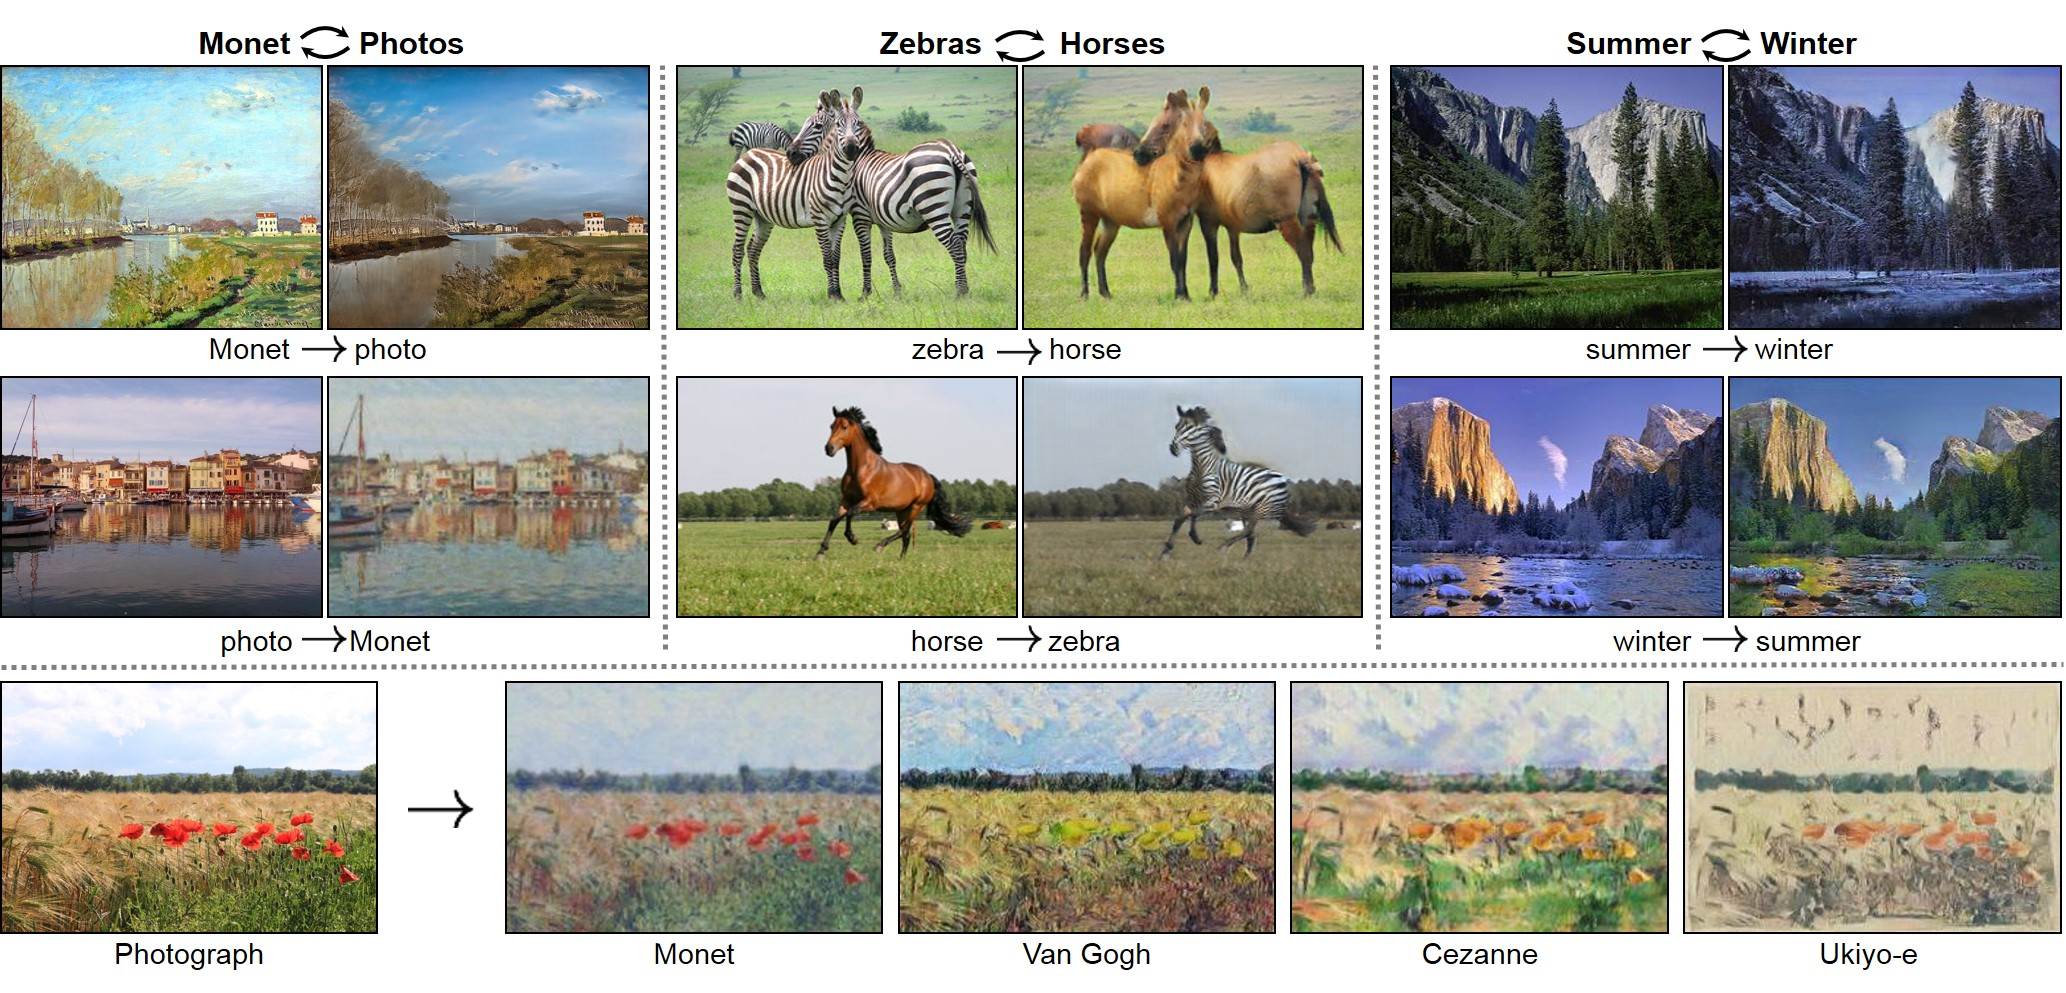
\includegraphics[width=\linewidth]{images/cyclegan.jpg}
            \caption{Pildi muundamine}
            \label{fig:cyclegan}
    \end{figure}
    CycleGAN on GAN, mis lahendab pildi pildiks teisendamise probleemi ehk teisendades pildi ühes stseeni representatsioonist $ x $ teise $ y $. Näiteks teisendades mustvalgepilt värviliseks pildiks või teisendades õhufoto kaardiks. Varasemad meetodid on ainult töödanud olukordades, kus on olemas pildipaarid $ \left\{x_i,y_i\right\}_{i=1}^N $. Pildipaaride kogumine on aga kallis ning keeruline, selle tõttu on valmis andmekogumid pildi paaridest väikesed.

    
    CycleGANi on võimalik treenida teisendaa pilte erinevate domeenide vahel, kus puuduvad pildipaarid

    Olgu meil pildikogum $ X $ ja teine kogum $ Y $. Me võime treenida seose $ G: X \rightarrow Y $ nii et väljund $ \hat{y} = G(x), x \in X $ eristamatu piltidest ja $ y \in Y $ kasutades vastast, mis on treenitud eristama $ \hat{y} y $-st.
    Seega $ G $ teisendab domeeni $ X $ domeeni $ \hat{Y} $, mis on jaotatud samamoodi nagu $ Y $. See aga ei garanteeri, et sisend $ x $ ja väljund $ y $ on seotud paari tähendusrikkal viisil --- on olemas lõpmatult palju teisendusi, mis tekitavad sama jaotuse üle $ \hat{y} $.

    Probleem lahendub kui lisada eesmrägile lisa tingimus, et teisendus peab olema tsükkliliselt järjepidev. Näiteks kui tõlkida lause eesti keelest inglise keelde, siis tagasi tõlkides peaks jõudma tagasi algse lauseni. Matemaatiliselt kui on teisendus $ G: X \rightarrow Y $ ja teine teisendus $F: Y \rightarrow X $, siis peaksid $ G $ ja $ F $ olema üksteise pöördfunktsioonid.
    Seda saab rakendada treenides teisendusi G ja F samaaegselt ning lisades tsüklilise järjepidevus kao, mis motiveerib et $ F(G(x)) \approx x $ ja $ G(F(y)) \approx y $. Kombineerides selle kao koos vastandliku kaoga domeenides $ X $ ja $ Y $, annab täis eesmärgi mitte paaris piltite teisenduseks.

    \subsection{AttnGAN}
    \subsection{Mudel}
    Kasutades AttnGANi ja CycleGANi, on võimalik muuta tekst kunstiks --- sisendiks võetakse tekst, mis kirjeldab pildi sisu, ning lisaks number, mis ütleb, mis stiilis pilti genereerida. Tekst antakse sisendiks AttnGANile, mis muudab selle pildiks, ning seejärel valitakse stiilile vastav CycleGAN, mis muudab ennem loodud pildi kunstiteoseks.


    \section{Eksperimendid}

    \unsection{Kokkuvõte}
    \unsection{Summary}

    % The bibliography
    \nocite{*} % List all entries, even when not cited
    \printbibliography[title={Kasutatud allikad}]

\end{document}
